\chapter{Mesh-sweeping for sparse manifold refinement}
\label{ch:sweeping}

In the previous chapter we show that the output of the 3D reconstruction from Sparse Points represents a good candidate to initialize the surface evolution algorithm which is able to reconstruct the details of the scene. 
In this chapter we investigate how to to improve the accuracy and the convergence of the surface evolution algorithm. 
In particular we guess that a better manifold reconstruction would lead to this improvement. 
Therefore, we propose to add a limited but very precise set of new points to the sparse point cloud we use as a support for the 3D reconstruction. 
The method fits in the framework presented in the former chapter, it keeps the manifoldness and it lets the pipeline to be completely automatic.


\minitoc
\newpage

\section{Rationale}

Reconstructing the observed scene from a set of images is a widely studied problems in computer vision: it is known as \emph{Structure from Motion} (SfM), when the aim is to reconstruct both the scene (the structure) and the camera poses (the motion), or as \emph{multi-view stereo} (MVS), when camera poses are known.
While SfM techniques provide a sparse reconstruction of the environment, MVS aims at reconstructing a dense and accurate model of the observed scene. 

Since the datasets of \cite{seitz_et_al06} and \cite{strecha2008} were made available, dense MVS has been faced with different approaches, some of which reaching very accurate results, but some issues are still open, e.g., the initialization and the management of untextured regions and false matches.
Mesh-based methods have been proven to be suitable to build continuous, high accurate reconstructions of both small objects and large-scale scenes \cite{hiep2009towards,vu_et_al_2012,salman2010surface}.
These methods refine an existing mesh by minimizing an image similarity measure such as the Zero Mean Cross Correlation (ZNCC) \cite{hiep2009towards,pons2007multi,zaharescu2007transformesh} or the Sum of Squared Differences (SSD) \cite{delaunoy_et_al_08,delaunoy2011gradient}. 
The initialization of this existing mesh is one of the major issues in the state-of-the-art mesh-based MVS methods. For single object reconstruction, as in the Middelbury dataset \cite{seitz_et_al06}, the initial mesh is usually estimated by the visual hull \cite{laurentini1994visual}, but this is not applicable in more complex scene such as the ones in \cite{strecha2008} or in large-scale scenarios.

One of the most effective and scalable mesh-based algorithm for multi-view stereo was proposed by Vu \emph{et al}. \cite{vu_et_al_2012}; in their work, the authors initialize the mesh evolution algorithm by extracting a dense and noisy point cloud, building a Delaunay triangulation out of it, and estimating the initial mesh via a \emph{s-t} cut algorithm based on the work of \cite{labatut2007efficient}. 
This last work inspired other extensions such as \cite{jancosek2011multi}.
The main problem with this approach is that the \emph{s-t} cut does not guarantee the output mesh to be a manifold while the \emph{surface evolution} algorithm needs this property; indeed Vu \emph{et al}.  need to manually check the outcome of the \emph{s-t} cut before the surface evolution.

Some mesh-based algorithms, e.g., \cite{pan2015automatic,li2015detail}, initialize the reconstruction with a point-based MVS such as CMVS \cite{fu10} together with Poisson Reconstruction \cite{kazhdan2006poisson}.
This process automatically provides an initialization usually close to be manifold but not guaranteed, but it has issues related to redundancy of the points and non-scalability.

in the last chapter we presented a method   to estimate a manifold mesh  from sparse data which are the outcome of SfM algorithms. 
For many applications the reconstruction relying only on these points is sufficient, but for a surface evolution approach, an resolution and accuracy improvements bring to a faster and better convergence; indeed, Vu \emph{et al}. \cite{vu_et_al_2012} densify the point cloud extracted by the SfM algorithm too.

In this chapter we propose a novel and fully automatic approach to estimate a manifold, suitable for being a good initialization for a surface evolution mesh-based MVS algorithm.
We bootstrap from the manifold reconstructed from sparse points; we refine the mesh by iteratively sweeping its triangle facets around their neighborhood and we look for good stereo matches.
This approach takes inspiration from the multi-directions plane-sweep of \cite{gallup2007real}.
In \cite{gallup2007real}, the authors sweep a set of planes choosing fixed directions related to the direction of the walls identified from Structure from Motion points; for each pixel and each plane they collect the matching costs among the views and choose the best stereo matching cost to estimate depth maps.
Another interesting method that performs local plane sweeping is presented in \cite{sinha2014efficient}, where, again, the output is a depth map.
In the proposed approach, instead, we estimate directly a manifold mesh; the directions of the planes are automatically driven by the data; and we avoid to sweep on the whole scene, since we look for new 3D points in the neighborhood of the iteratively reconstructed manifold. 
Differently from \cite{gallup2007real}, we directly recover a consistent dense 3D mesh instead of independent depth maps.

\begin{figure}[t]
  \centering
  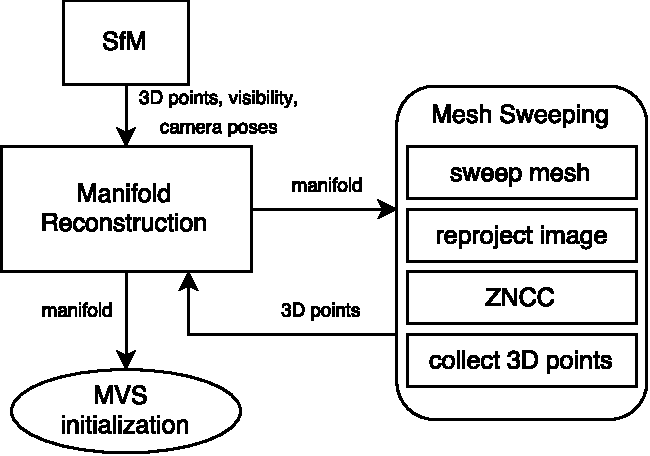
\includegraphics[width=0.9\columnwidth]{./img/ch-sweep/mesh-sweeping_overview}
\caption{Overview of the proposed algorithm.}
  \label{fig:overview}
\end{figure}


%------------------------------------------------------------------------- 
\section{System Overview}
\label{sec:overview_sweep}
In the proposed system we iteratively alternate between manifold reconstruction and mesh sweeping as illustrated in Figure \ref{fig:overview}.
The pipeline we propose takes into account all the SfM cameras and 3D points in the same time to focus the explanation on the mesh sweeping, however the formalization we provide, lets the algorithm to be easily applicable even in the general incremental setting.

We estimate the initial manifold mesh as described in the previous chapter by applying the   \emph{Point Insertion}, \emph{Ray tracing} and \emph{Growing} steps.
To enhance this manifold, we extract new 3D points by mesh sweeping, and we add them together with thei visibility to the manifol reconstruction algorithm which add them in the manifold by applying the \emph{Shrinking}, \emph{Point Insertion}, \emph{Ray tracing} and \emph{Growing} steps.


\begin{figure}[tp]
  \centering
  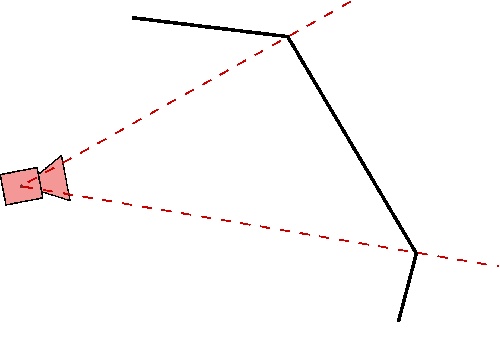
\includegraphics[width=0.8\textwidth]{././img/sweep.pdf}
  \caption{Example of manifold sweeping with respect to the camera $C$}
  \label{fig:sweep}
\end{figure}


\begin{figure}[tp]
  \centering
  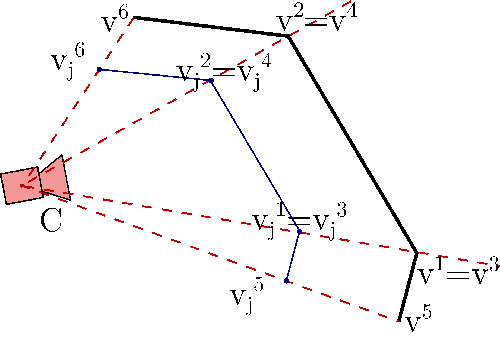
\includegraphics[width=0.8\textwidth]{./img/ch-sweep/sweepMulti.pdf}
  \caption{Sweeping of all the facets of the mesh with respect to the camera $C$}
  \label{fig:sweepMulti}
\end{figure}


 

%------------------------------------------------------------------------- 
\subsection{Mesh Sweeping}
\label{sec:sweep}
The novel mesh sweeping algorithm looks for new 3D points in the neighborhood of the manifold mesh, which we assume to be close to the true model of the scene.
These points will be added to the reconstruction in the next manifold reconstruction step.

The mesh sweeping acts on pairs of cameras: a reference  and a comparison camera. 
For a reference camera $C$, we sweep the visible part of mesh $\mathcal{M}$ along the viewpoint direction (see Figure \ref{fig:sweep}). 
Given a camera located in $C$, we sweep each visible facet $f$ of $\mathcal{M}$ by an amount multiple of $\alpha$ (in our case $\alpha = 3$cm).
Let $v^1$, $v^2$ and $v^3$ be the vertices of $f$, and let $\theta^i$ be the angle between the normal $n$ of the facet and the ray $d^i$ from the camera center to the vertex $v^i$. 
The new vertex $v_j^i$ of the swept facet is now computed as:
\begin{equation}
v_j^i = v^i + \alpha_j \, \cos (\theta^i) \, d^i,
\end{equation}
where $\alpha_j = \alpha  k_j$, with $k_j \in \mathbb{N}$ and $-10< k_j <10$ is the distance swept (let note that is fixed for all the facets).

Let notice that all the visible vertices of each triangle are swept by the same amount along the camera-to-point direction. 
Therefore the connectivity of the mesh is preserved \ie the corresponding vertices of the swept facets coincide (see Figure \ref{fig:sweepMulti}),  and no self-intersections among facets has been induced. 

We apply the previous process for each input camera, considered as a reference, that we compare with the two nearest cameras of the sequence.



\begin{figure}[t]
\centering
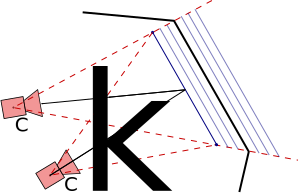
\includegraphics[width=0.8\textwidth]{./img/sweepSteps-01}
\caption{Reprojection of image $I_k$ on camera $C$ through one of the mesh triangle.}
\label{fig:stereo}
\end{figure}

\begin{figure}[t]
  \centering
  \includegraphics[width=0.8\textwidth]{././img/matching.pdf}
\caption{3D points extraction process after the mesh sweeping.}
  \label{fig:matching}
\end{figure}


The sweeping process produces a set of $N = 20$ meshes:
\[
    \mathbb{M} = \{\mathcal{M}_1, \cdots, \mathcal{M}_j ,\cdots, \mathcal{M}_N\}.
\]
For each mesh $\mathcal{M}_j$ we perform pairwise stereo matching between each camera $C$ and the two nearest cameras.
Let $I_C$ be the image seen by $C$, and $I_k$ the image seen by the camera $C_k$, that is one of the two cameras nearest to $C$. 
We compute $I_k^j$ as the reprojection of image $I_k$ through the mesh $\mathcal{M}_j$ into camera $C$.

% We store in a second image $P_k^j$ the 3D position of the points that reproject for each pixels, such that $P_k^j(x,y)$ stores the 3D point nearest to camera $C$ that reprojects on pixel $(x,y)$.

Then, we compute  the Normalized Cross Correlation (NCC) image $I_C$ and the reprojection $I_k^j$. 
The NCC is computed pixel-by-pixel and is weighted by a Gaussian kernel as in \cite{pons2007multi}  (the $\sigma$ for the Gaussian kernel is $\sigma = 8 px$).

The last step aims at collecting the new 3D points. We create a $n_r$x$n_c$ grid over the $N$ images of pixel-by-pixel NCCs computed for each mesh $\mathcal{M}_j$. We collect in each tile the image point with the best NCC above a threshold $t_{\text{NCC}} = 0.98$ among all the $N$ images; therefore, we obtain at most $n_r$x$n_c$ points.
For each collected point, we retrieve its 3D position from the corresponding mesh that generated it.

We are able to perform the whole process image-based, i.e., we act on the image and not on the mesh, so that the most complex computations become independent from the size of the mesh, and they are self-adaptive with respect to the  image resolution. This also allows our approach to be adaptive in term of mesh resolution output.

\begin{figure}[tp]
\centering
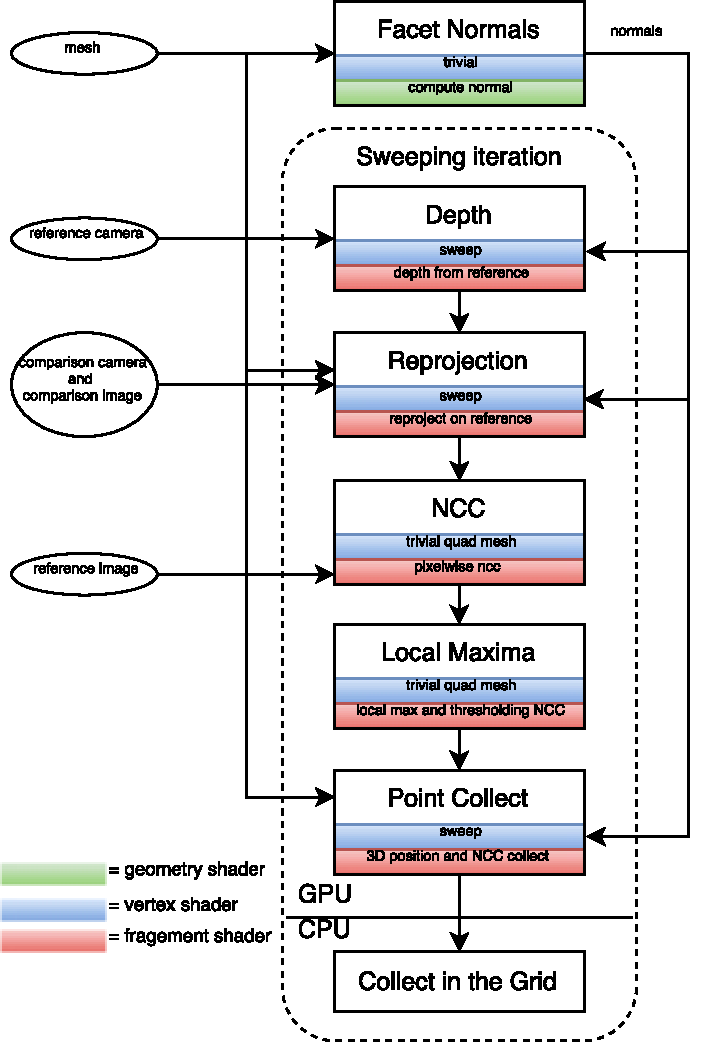
\includegraphics[height=0.99\textheight]{./img/ch-sweep/Sweep-shaders-architecture}
\caption{Architecture of the sweeping algorithm.}
\label{fig:sweep-arch}
\end{figure}

\section{Implementation details}
We implemented our approach in C++ using the CGAL library \cite{cgal} for all the computations involving the Delaunay Triangulation and manifold extraction. This allows us to exploit efficiently data structures and algorithms for the initial manifold reconstruction tasks: thanks to the 3D triangulation module, we managed to encode all the visibility information inside each tetrahedron.

Conversely, the proposed mesh sweeping algorithms exploits the power of GPU computing. 
\subsection{Shaders architecture}
We implemented the main steps with the GLSL shading language of OpenGL \cite{opengl} to exploit the parallelism of GPU computing.
The modern openGL architectures are organized in blocks made up of:
\begin{itemize}
 \item a vertex shader, which processes each vertex of the mesh and, in its basic usage, it computes their positions in the image plane;
 \item an optional geometry shader, which processes the whole infomation of the vertices for each facet of the mesh
 \item a fragment shader, which is dedicated to compute the color of each pixel of the rendered image.
\end{itemize}
Our algorithm well fits into this programming framework: in Figure \ref{fig:sweep-arch} we show the details of the architecture of the mesh sweeping. 

First, we send to GPU the entire mesh visible from the current reference camera and we compute the normals of the facets with a geometry shader, in this case we do not need to render any image therefore the vertex shader acts just to transfer vertex position, while the fragment shader remain unused.
Then we iterate for each $\alpha_j$ value the core algorithm. 
We compute the depth useful to get rid of occlusions in the reprojection ste in which the image of the second camera is projected on the through the mesh to the image plane of the reference camera. 
This two blocks shares the same vertex shader which sweeps the mesh in the 3D space; and the respective fragment shaders computes the pixel-per-pixel depth of the mesh with respect to the reference camera, and the color of the reprojection in the reference camera.
The following block compute the NCC between the reference image and the output of the reprojection shaders: in this case the computations are performed directly on the images, therefore the vertex shader projects a trivial quad mesh that covers the image plane, where the fragment shaders compute the NCC for each pixel.
The local maxima block is image based too, and lock for very good NCC values in the output of the previous step: here the fragment shader render a non-zero pixel where the NCC value is greater than $t_{\text{NCC}}$ and is greater of all the values in its neighborhood (a $\sigma x \sigma$ squared window), otherwise it puts the value to $0$.
Eventually, the last block collects the 3D positions where high NCC have been found: the vertex shader compute the sweept mesh and its projection on the reference image, the fragment shader encodes the 3D position in the first three channel of pixel where the output of the previous step is a non-zero value and populate the foruth channel with the NCC value itself.
In the last step we dump the pixel on the CPU and we collect them into the $n_r$x$n_c$ grid, keeping the 3D point with the best NCC for each tile.



\section{Experimental validation}
The proposed algorithm provides an automatic initialization for mesh-based dense MVS algorithms.
We implemented our approach in C++ using the CGAL library \cite{cgal} for all the computations involving the Delaunay Triangulation and manifold extraction. This allows us to exploit efficiently data structures and algorithms for the initial manifold reconstruction tasks.
Conversely, the proposed mesh sweeping algorithms exploits the power of GPU computing; we implemented the main steps with the GLSL shading language of OpenGL \cite{opengl}: a geometry shader computes the normal; the vertex shaders sweep the mesh along the camera viewing rays; the fragment shaders implement the reprojection from one image to an another through the mesh surface, the NCC computation and thresholding.


We performed experiments on both synthetic and real datasets on a 4 Core i7-2630QM CPU at 2.2Ghz (6M Cache), with 6GB of DDR3 SDRAM and NVIDIA GeForce GT 630M. The former experiments aim at showing the effectiveness of the mesh sweeping approach to refine a rough manifold.
The experiments on real data show the scalability of the proposed method and its effectiveness compared to CMVS \cite{fu10}, used as automatic initialization in mesh-based algorithms as \cite{pan2015automatic,li2015detail} together with Poisson reconstruction \cite{kazhdan2006poisson}. 

\subsection{Synthetic Dataset}
In Figure \ref{fig:simulated1} we provide quantitative evaluation for two synthetic datasets.
The ground-truth meshes we used to generate the image are two pyramids without the squared base (Figure \ref{fig:simulated1}(b)), pointing downward for the first dataset, and upward in the second one; the dimensions of these pyramid are 2x2m of squared base and 0.3m height.
The initial point cloud in both cases is made up by the four vertices of the base. 
We bootstraps from only these four points, to show the impact of the proposed approach even if few sparse points are available.
In both cases the initial manifold extracted is a square corresponding to the base of the pyramid (Figure \ref{fig:simulated1}(c)).
The final reconstructions are shown in Figure \ref{fig:simulated1}(d) even if some little artifacts are created due to the noise in the matching process, the extracted surface is close to the ground-truth.
We computed the distance of the meshes with respect to the ground truth by comparing the depth of each pixel from the first camera, similarly to the comparison method proposed in \cite{strecha2008}. 
In Table \ref{tab:resSim} we compare the accuracy of the initial mesh with the accuracy after the proposed mesh sweeping: our method improves significantly the initial mesh; this result is also supported by the improvement on the error distributions in  Figure \ref{fig:simulatedhist} and \ref{fig:simulatedhist2}.
In Table \ref{tab:resSimImp} we applied the photometric refinement of \cite{vu_et_al_2012} to the two meshes and we shows the results: the convergence of the refinement after the mesh sweeping is faster and the the reconstruction more accurate.


\begin{figure}[th]
\setlength{\tabcolsep}{1px}
\centering
\begin{tabular}{ccccc}
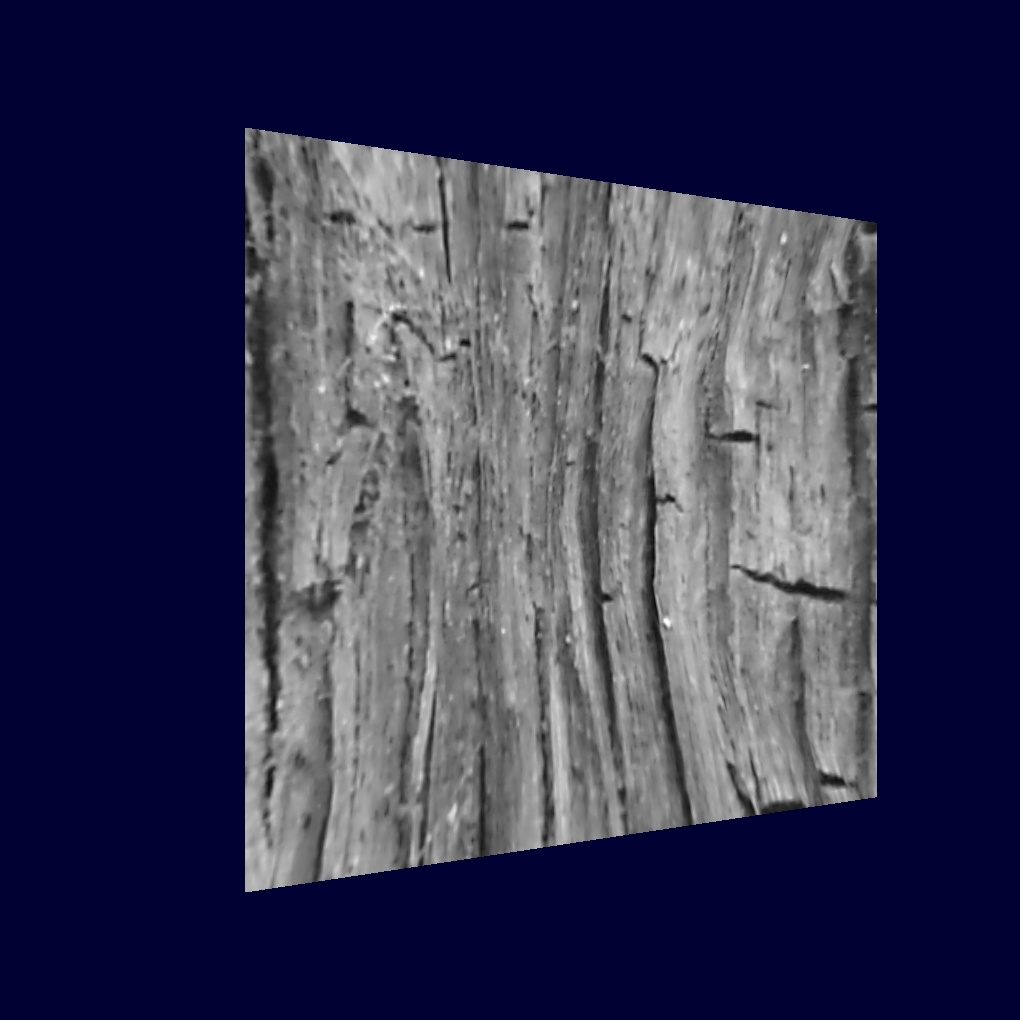
\includegraphics[height=0.18\textwidth]{./img/datasetSweepIMG0}&
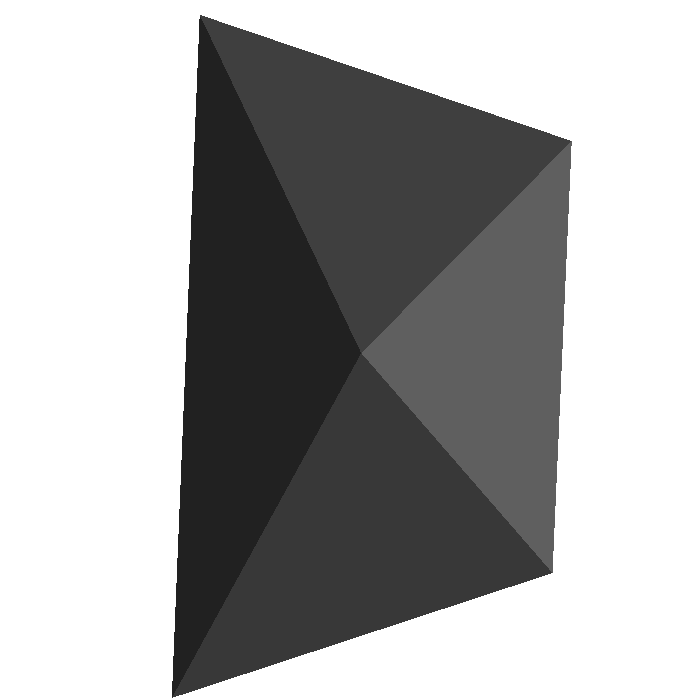
\includegraphics[height=0.18\textwidth]{./img/synthGT1}&
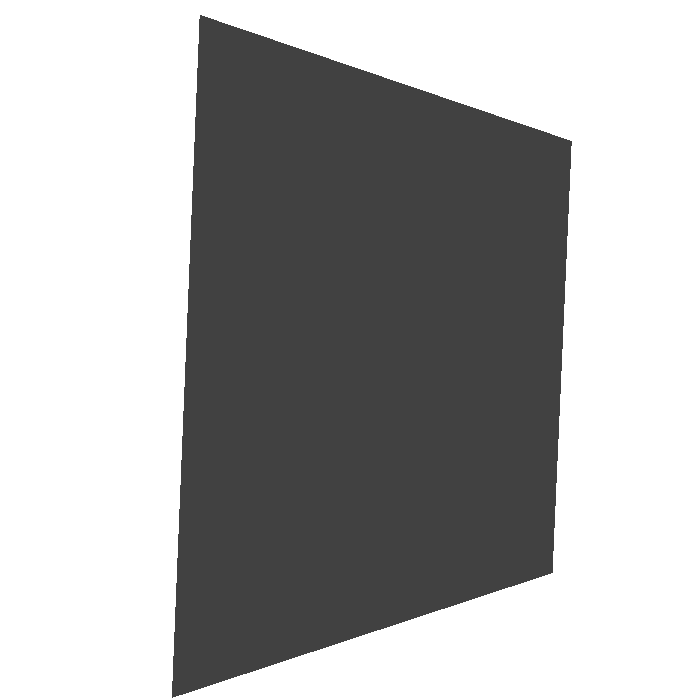
\includegraphics[height=0.18\textwidth]{./img/synthInit1}&
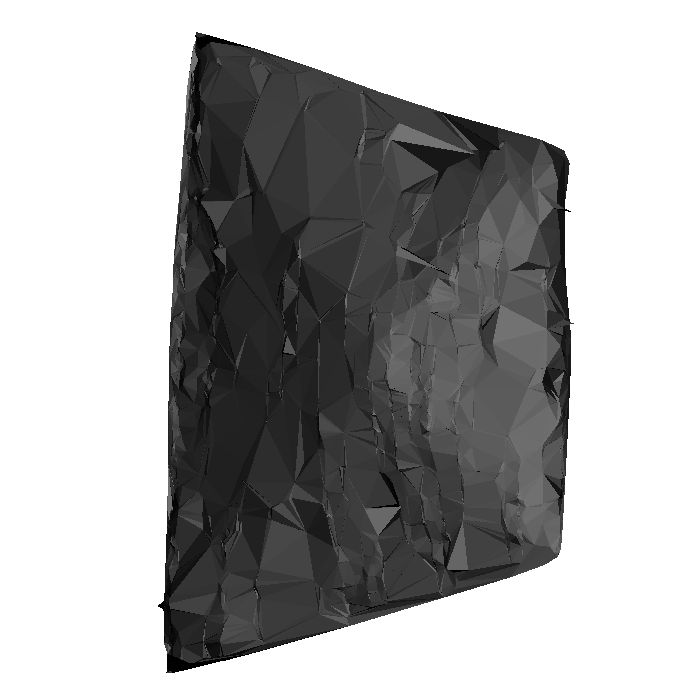
\includegraphics[height=0.18\textwidth]{./img/synthNOtRef1}&
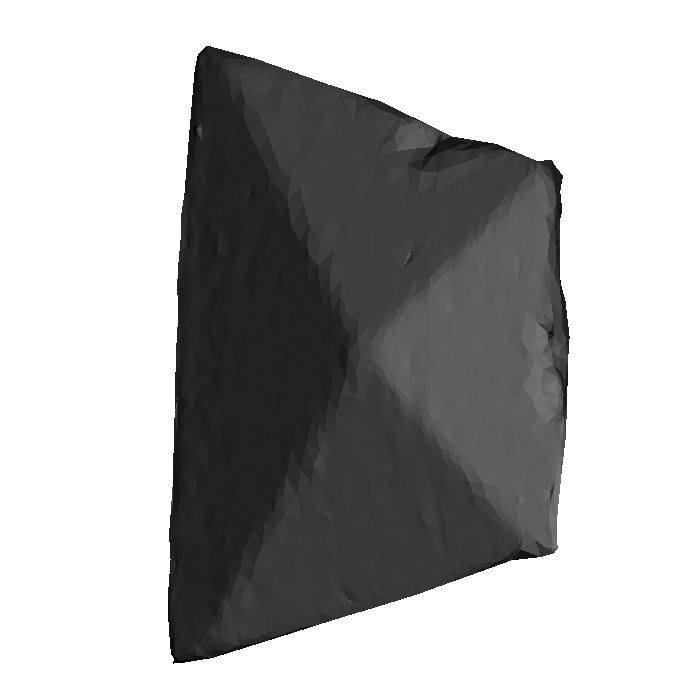
\includegraphics[height=0.18\textwidth]{./img/synthRef1}\\
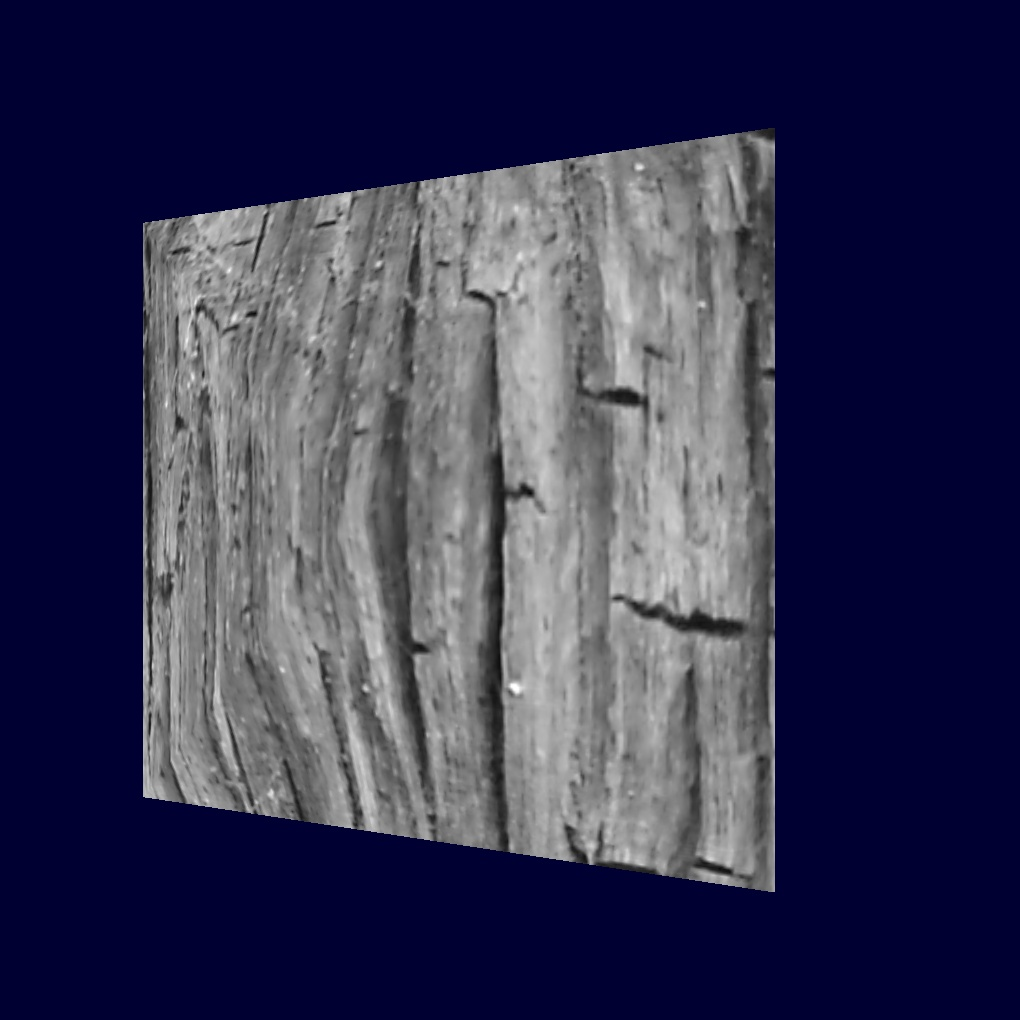
\includegraphics[height=0.18\textwidth]{./img/datasetSweepIMG1synth2}&
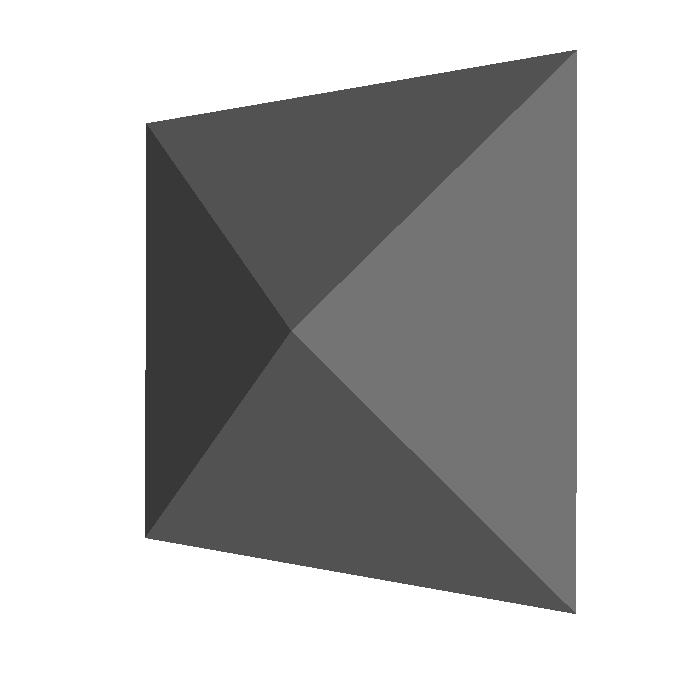
\includegraphics[height=0.18\textwidth]{./img/synth2_GT}&
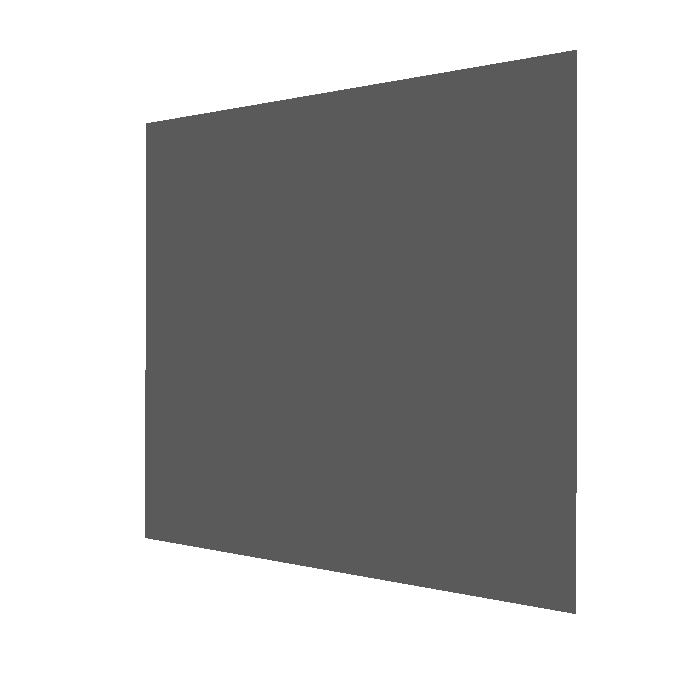
\includegraphics[height=0.18\textwidth]{./img/synth2_init}&
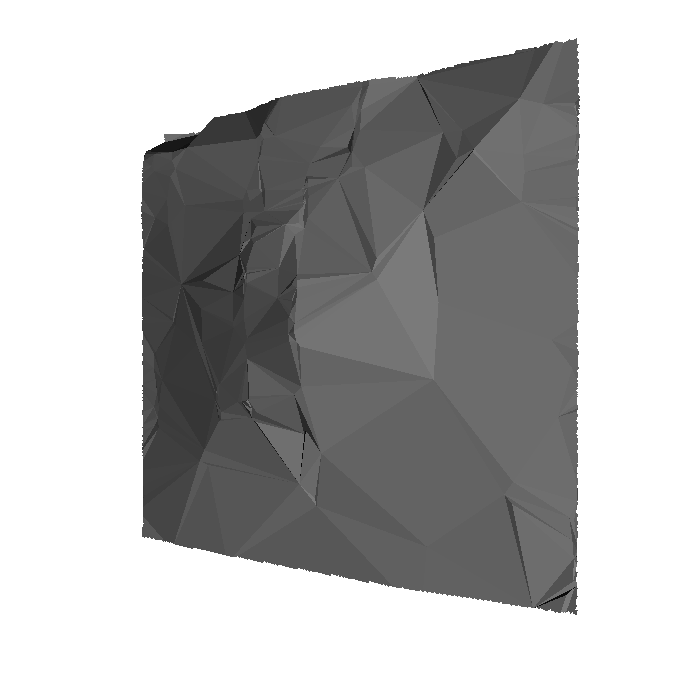
\includegraphics[height=0.18\textwidth]{./img/synth2_after_sweep}&
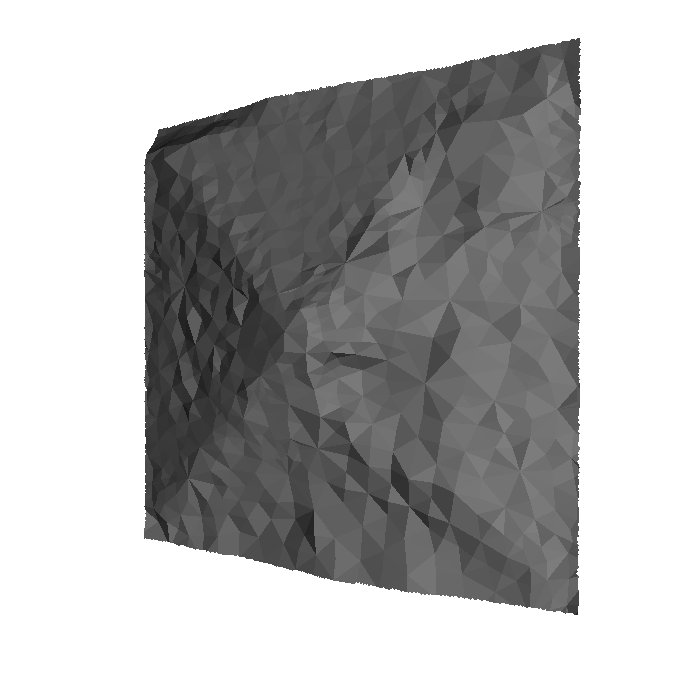
\includegraphics[height=0.18\textwidth]{./img/synth2_after_photo}\\
(a) &
(b)&
(c) &
(d) &
(e)\\
\end{tabular}
\caption{Simulated dataset results: (a) textured image, (b) ground-truth, (c) initial mesh, (d) after mesh sweeping, (e) after photometric refinement.}
\label{fig:simulated1}
\end{figure}

%In these experiments, we include the approach to deal with untextured regions and, as expected we notice no negative influence in these textured dataset.

\begin{figure*}[t]
\setlength{\tabcolsep}{1px}
\centering
\begin{tabular}{cc}
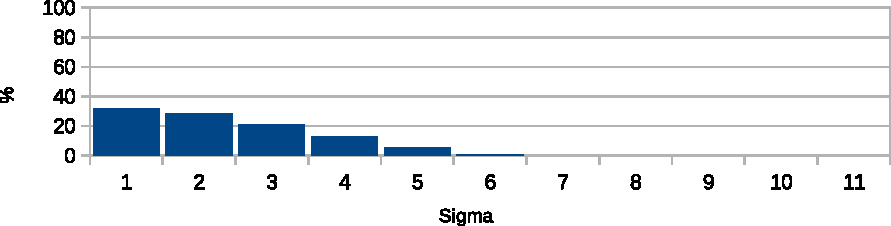
\includegraphics[width=0.49\textwidth]{./img/synth1InitHist}&
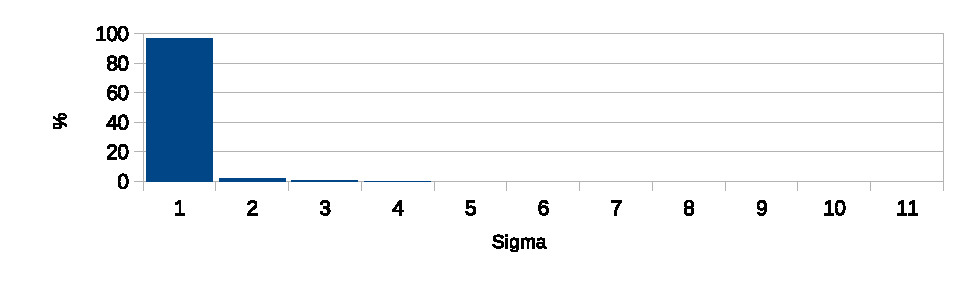
\includegraphics[width=0.49\textwidth]{./img/synth1ResHist}\\
\multicolumn{2}{c}{Synthetic Dataset 1}\\
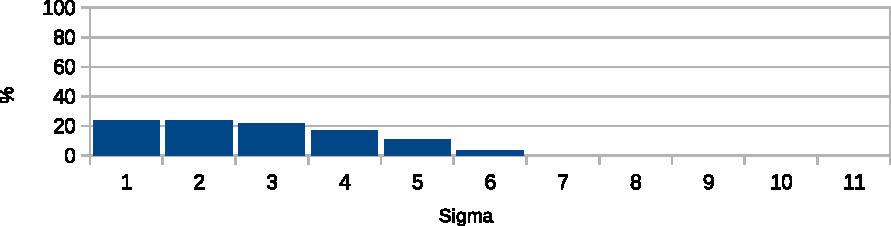
\includegraphics[width=0.49\textwidth]{./img/synth2InitHist}&
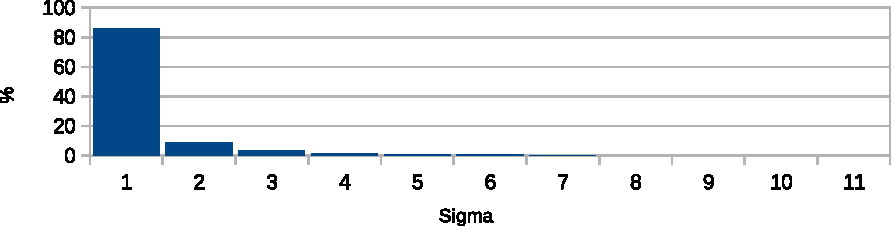
\includegraphics[width=0.49\textwidth]{./img/synth2ResHist}\\
\multicolumn{2}{c}{Synthetic Dataset 2}\\
(a) &
(b) \\
\end{tabular}
\caption{Histograms of errors in synthetic dataset: (a) initial manifold, (b) final manifold (Sigma = 0.06m).}
\label{fig:simulatedhist}
\end{figure*}


\subsection{Real Dataset}
We tested the proposed approach on the \emph{fountain-P11} dataset provided in \cite{strecha2008}: the ground-truth is available and the evaluation is performed by comparing the depth map generated from the 6th point of view as suggested in  \cite{strecha2008}, such that the results of the comparison are independent from the quality of the camera calibration (a detailed discussion is available in \cite{strecha2008}). We initialized the manifold reconstruction with the sparse point cloud data estimated with VisualSFM \cite{wu2011visualsfm}. 


Table \ref{tab:resFount} shows the accuracy of the initial manifold, estimated in a similar fashion to \cite{romanoni15b}, the manifold after the mesh sweeping and the reconstruction performed by CMVS+Poisson, where the octree depth of the Poisson reconstruction is 11 (see \cite{kazhdan2006poisson}). In Figure \ref{fig:fountainhist} we report the cumulative distribution of the errors for each algorithm.
As Figure \ref{fig:fountainIm} shows, the initial manifold represents accurately the wall, while some parts of the fountain present artifacts, indeed, the accuracy of this initial guess is lower than the outcome of CMVS+Poisson.
The mesh sweeping refinement improves the mesh accuracy, both respect to the initial mesh and to CMVS+Poisson reconstruction, even if the resolution of the latter is significantly higher. Our approach avoids to reconstruct redundant data, differently from the point-based CMVS, which reconstruct as much points as possible, even if they are coplanar.
Table \ref{tab:resFountPhoto} shows that the proposed approach improves the convergence of the variational photometric refinement described in \cite{vu_et_al_2012} leading to a more accurate reconstruction. 
The mean timing per-iteration is 318s for mesh sweeping and 55s for manifold reconstruction: the mesh sweeping is the most demanding task, but thanks to its GPU implementation it would easily take advantage from more powerful hardware.

Finally we tested the scalability of the proposed approach with a real dataset, named Dagstuhl, of 68 $1600\text{x}1200$ images (see Figure \ref{fig:Dagstuhl}). 
We tested the algorithm considering different subsets of frames to understand experimentally the dependence with the number of cameras of the proposed algorithm and the two steps (manifold reconstruction and mesh sweeping) separately. 
As Figure \ref{fig:scalability} points out, both steps and the whole algorithm show experimentally a linear relation with the number of cameras; this suggests that our approach is scalable and suitable for large-scene reconstructions.



\begin{figure}[t]
\setlength{\tabcolsep}{1px}
\centering
\begin{tabular}{c}
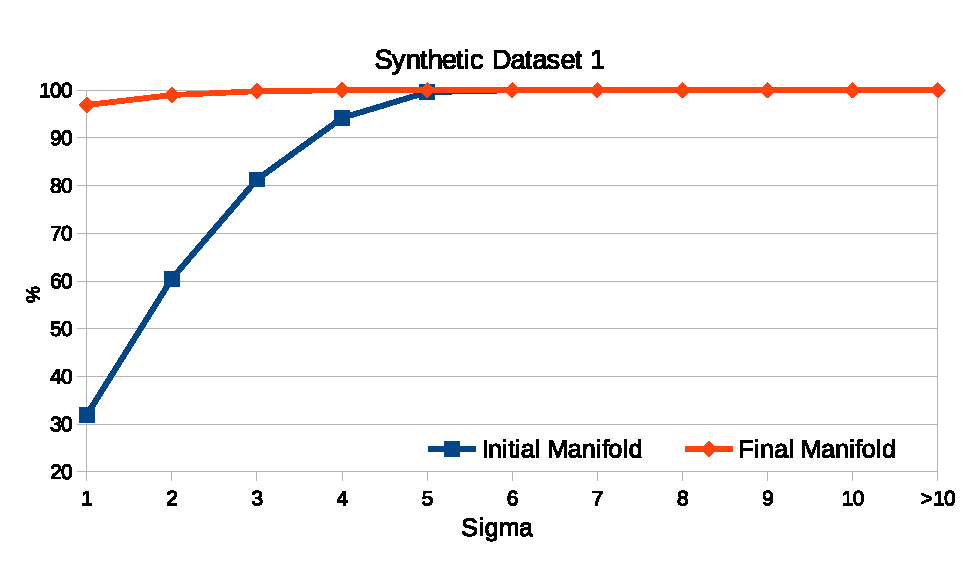
\includegraphics[width=0.48\textwidth]{./img/histSim1}\\
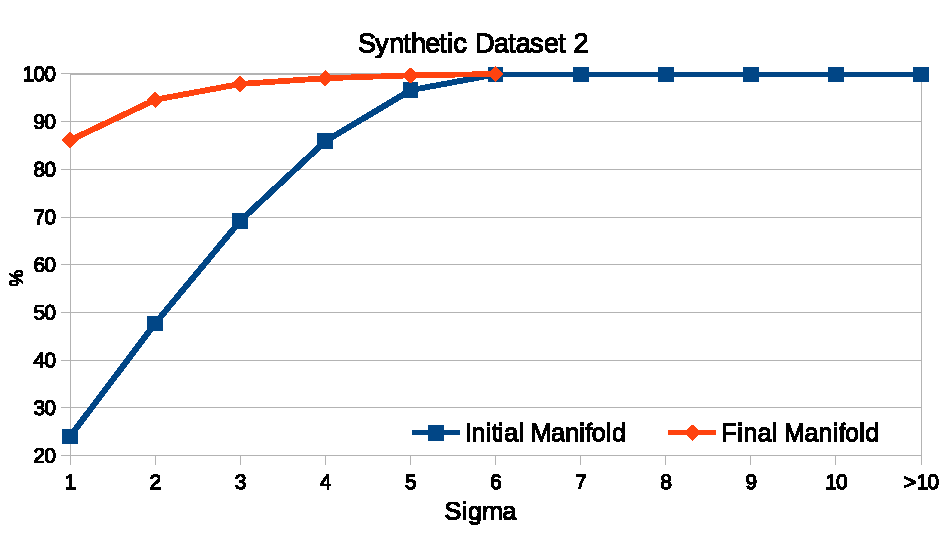
\includegraphics[width=0.48\textwidth]{./img/histSim2}\\
\end{tabular}
\caption{Cumulative distributions of error in the synthetic datasets (Sigma = 0.06m).}
\label{fig:simulatedhist2}
\end{figure}

\begin{table}[t]
\caption{Results of the proposed mesh sweeping in the synthetic datasets. All errors are in meters.}
\label{tab:resSim}
%\setlength{\tabcolsep}{1px}
\scriptsize
\centering
\begin{tabular}{lcccccc}
\toprule 
&\multicolumn{3}{c}{Downward Pyramid}&\multicolumn{3}{c}{Upward Pyramid}\\
              & MEA & MRE & RMS  &  MEA& MRE & RMS  \\
\midrule
w/o mesh sweeping  & 0.108 & 0.072 & 0.131 &  0.135 & 0.114 & 0.159 \\
w/ mesh sweeping    & 0.013 & 0.008 & 0.025 &  0.028 & 0.022 & 0.049 \\
improvement   & 88 \% & 89 \% & 81 \% &  79 \% & 81 \% & 69 \% \\
\end{tabular}
\end{table}


\begin{table}[t]
\caption{Photometric refinement with or without the mesh sweeping  in the synthetic datasets. All errors are in meters.}
\label{tab:resSimImp}
%\setlength{\tabcolsep}{1px}
\setlength{\tabcolsep}{4px}
\scriptsize
\centering
\begin{tabular}{lcccc|ccc}
\toprule 
&&\multicolumn{3}{c}{Downward Pyramid}&\multicolumn{3}{c}{Upward Pyramid}\\
Initial mesh & n. iter & MEA & MRE & RMS  &  MEA& MRE & RMS  \\
\midrule
w/o mesh sweeping &500 & 0.089 & 0.060 & 0.123 &  0.124 & 0.106 & 0.161 \\
w/o mesh sweeping & 5000 & 0.013 & 0.008 & 0.025 &  0.119 & 0.103 & 0.160 \\
w/ mesh sweeping &500& \textbf{0.002} & \textbf{0.001} & \textbf{0.008} &  \textbf{0.012} & \textbf{0.009} & \textbf{0.029} \\
\end{tabular}
\end{table}

% 
% \begin{figure*}[t]
% \setlength{\tabcolsep}{1px}
% \centering
% \begin{tabular}{ccc}
% 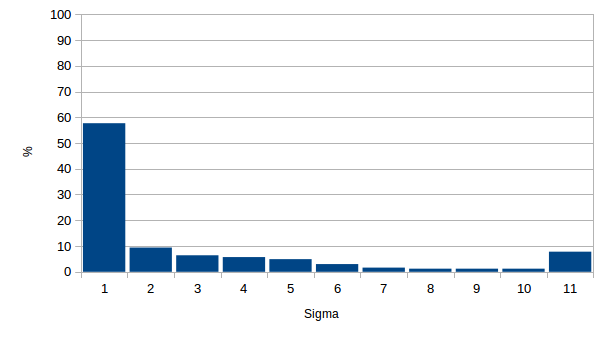
\includegraphics[width=0.32\textwidth,height=0.16\textwidth]{./img/poissonHist}&
% 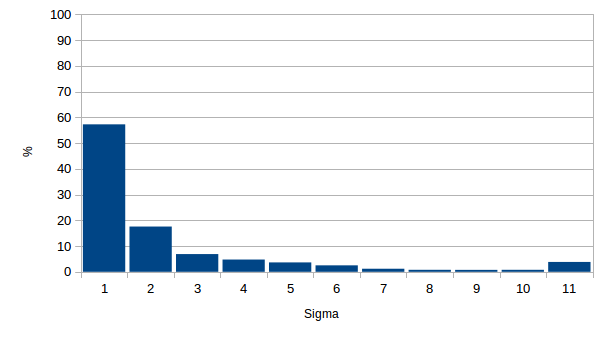
\includegraphics[width=0.32\textwidth,height=0.16\textwidth]{./img/realInitHist}&
% 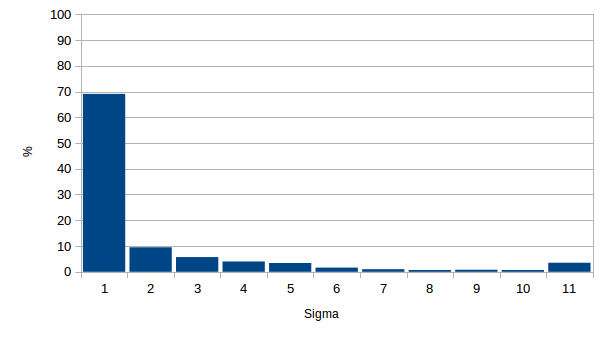
\includegraphics[width=0.32\textwidth,height=0.16\textwidth]{./img/realFinalHist}\\
% (CMVS+ Poisson) &
% (Initial manifold) &
% (Final manifold)\\
% \end{tabular}
% \caption{Histograms of errors in fountain-P11 dataset (Sigma = 0.06m).}
% \label{fig:fountainhist}
% \end{figure*}



\begin{table}[t]
\caption{Comparison between CMVS+Poisson, initial mesh and final mesh. Errors are expressed in Mean Absolute Error (MAE),  Mean Relative Error (MRE) and  Root Mean Square error (RMS).}
\label{tab:resFount}
%\setlength{\tabcolsep}{1px}
\scriptsize
\centering
\begin{tabular}{lcccc}
\toprule 
 & MEA & MRE & RMS & num. \\
 & (m) & (m) & (m) & vertices \\
\midrule
CMVS \cite{fu10} + Poisson  & 0.160 & 0.019 & 0.317& 253410\\
initial mesh \cite{romanoni15b} & 0.163 & 0.096 & 0.330 & 5880\\
final mesh (Proposed)  & \textbf{0.094} & \textbf{0.012} & \textbf{0.210} & 22336\\
\end{tabular}
\end{table}


\begin{table}[t]
\caption{Photometric refinement with or without the mesh sweeping  in the fountain dataset. All errors are in meters.}
\label{tab:resFountPhoto}
%\setlength{\tabcolsep}{1px}
\setlength{\tabcolsep}{4px}
\scriptsize
\centering
\begin{tabular}{lccccc}
\toprule 
Initial & & MEA & MRE & RMS & num. \\
mesh & n iter. & (m) & (m) & (m) & vertices \\
\midrule
w/o mesh sweeping &500& 0.130 & 0.157 & 0.304 & ~1M\\
w/ mesh sweeping &500& \textbf{0.069} & \textbf{0.008} & \textbf{0.196} & ~1M\\
\end{tabular}
\end{table}




\begin{figure}[t]
\centering
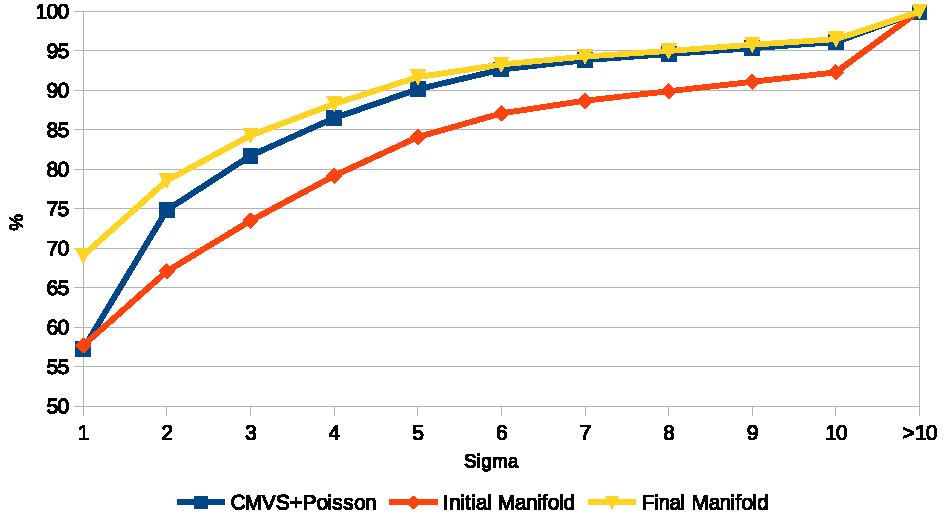
\includegraphics[width=\columnwidth]{./img/hist}
\caption{Cumulative distribution of errors in the fountain-P11 dataset (Sigma = 0.06m).}
\label{fig:fountainhist}
\end{figure}


\begin{figure}[t]
\setlength{\tabcolsep}{1px}
\centering
\begin{tabular}{cccc}
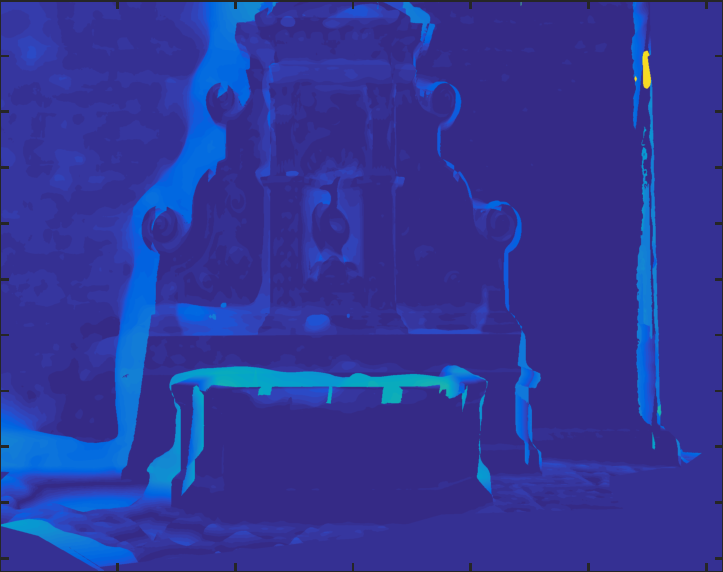
\includegraphics[width=0.25\columnwidth]{./img/errorPoisson}&
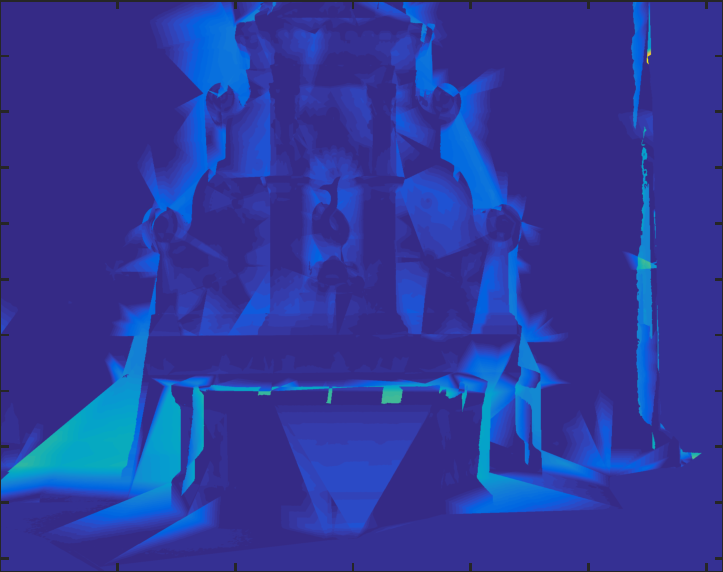
\includegraphics[width=0.25\columnwidth]{./img/errorMyFountainInit}&
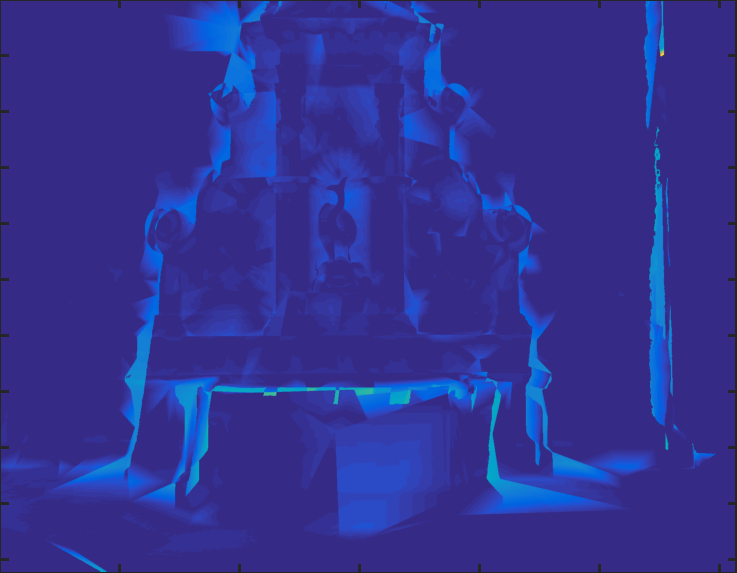
\includegraphics[width=0.25\columnwidth]{./img/errorMyFountainNotSm}&
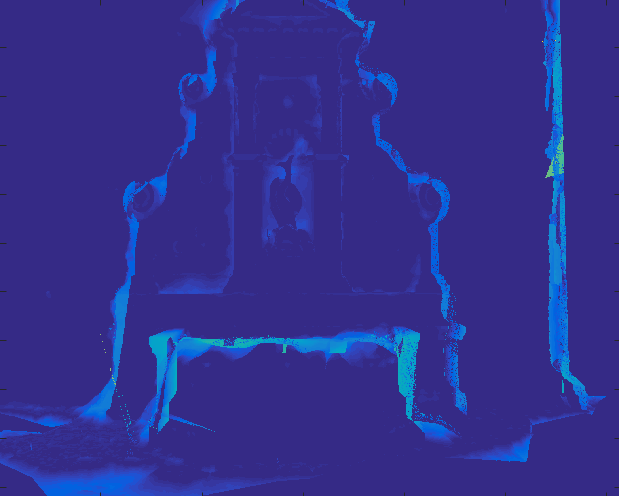
\includegraphics[width=0.25\columnwidth]{./img/Photofount}\\
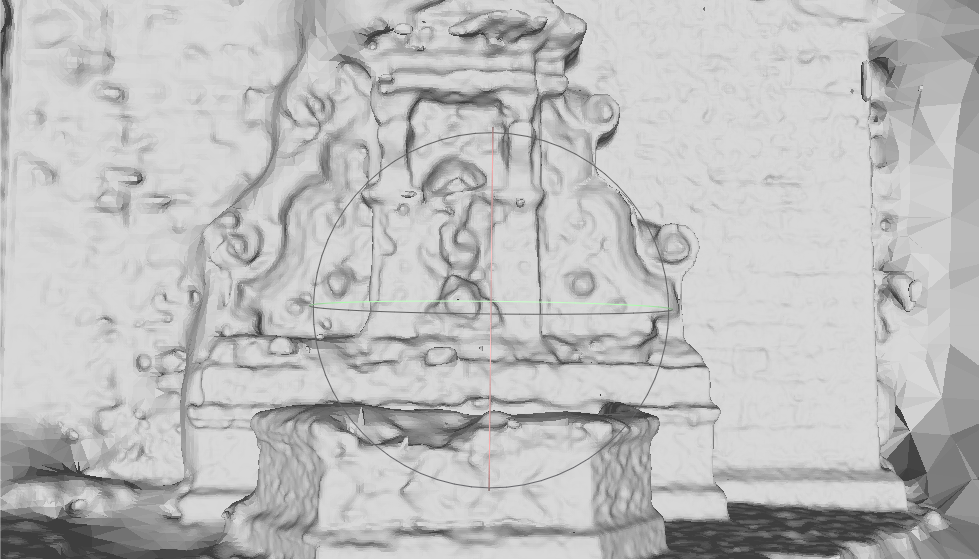
\includegraphics[width=0.25\columnwidth]{./img/poissonUntex}&
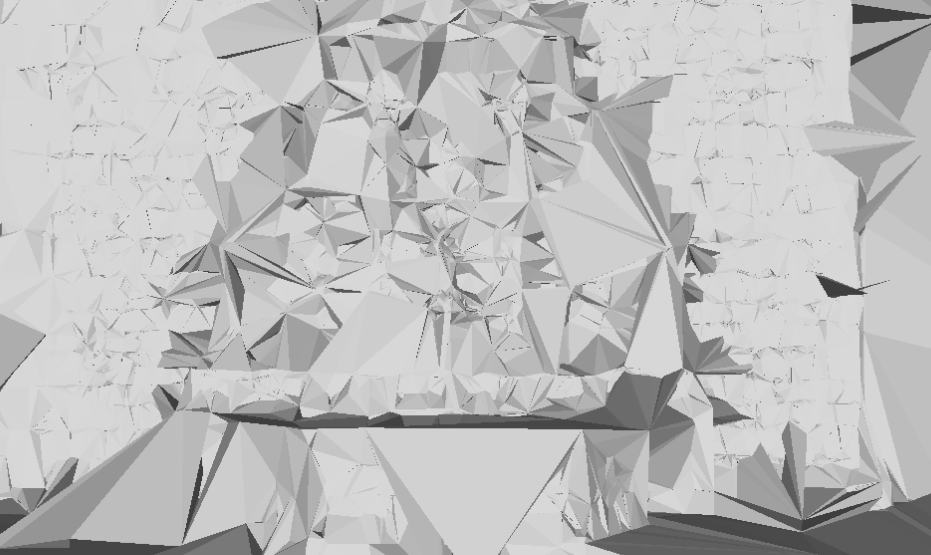
\includegraphics[width=0.25\columnwidth]{./img/firstUntex}&
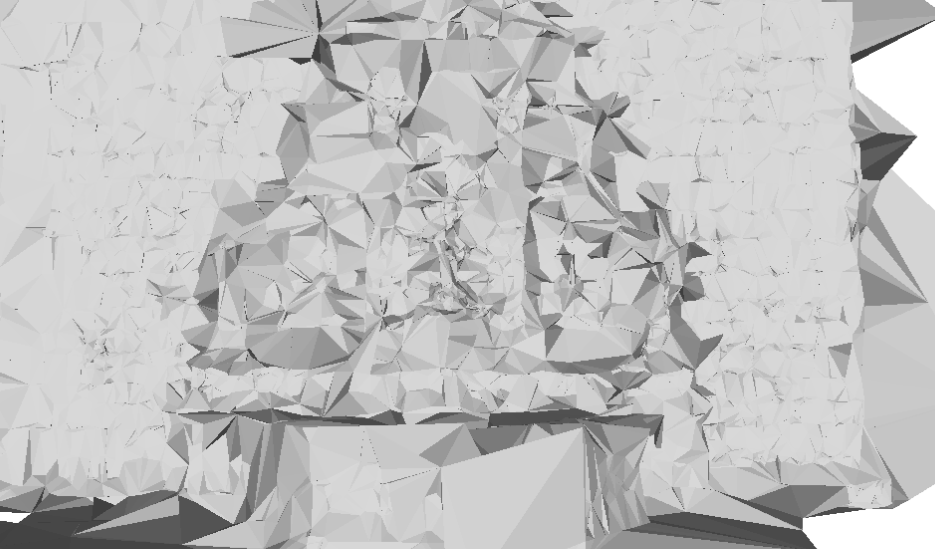
\includegraphics[width=0.25\columnwidth]{./img/myResUntex}&
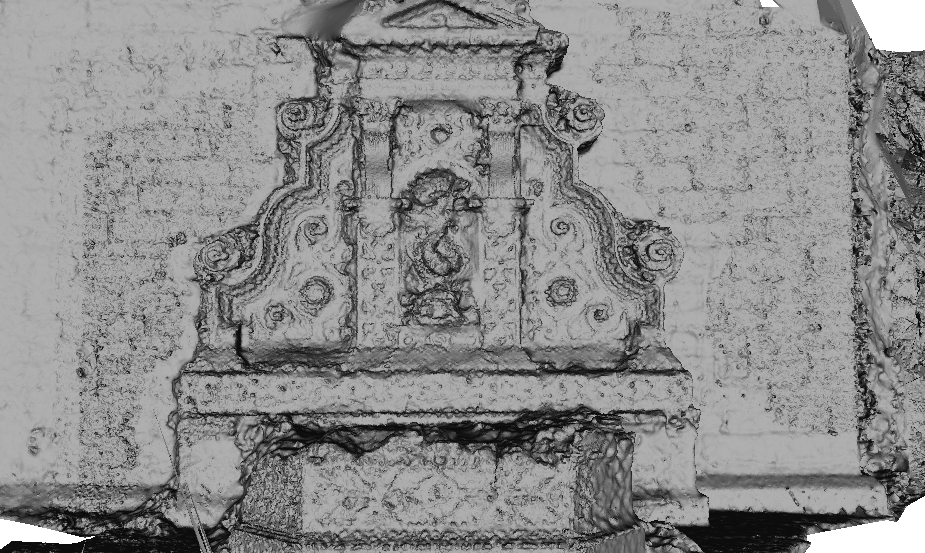
\includegraphics[width=0.25\columnwidth]{./img/photo_mesh_crop}\\
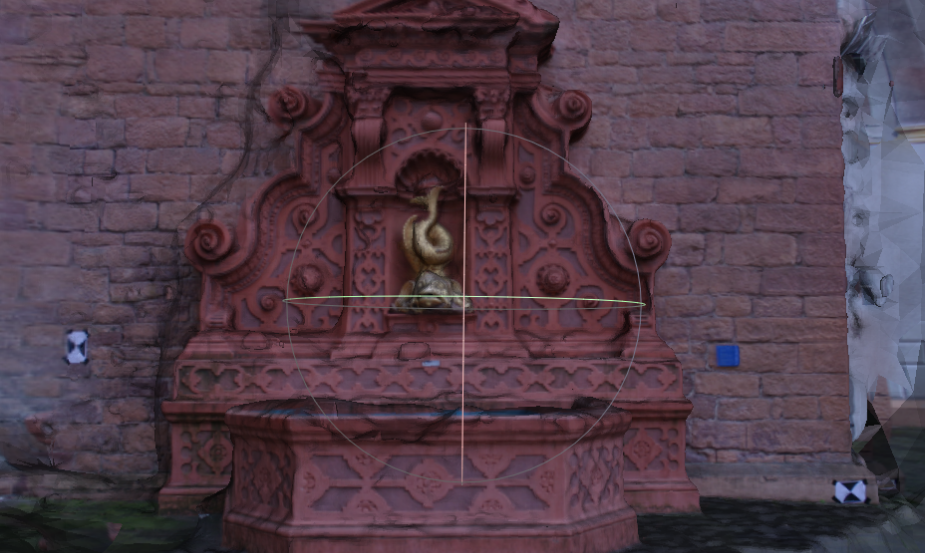
\includegraphics[width=0.25\columnwidth]{./img/poissonTex}&
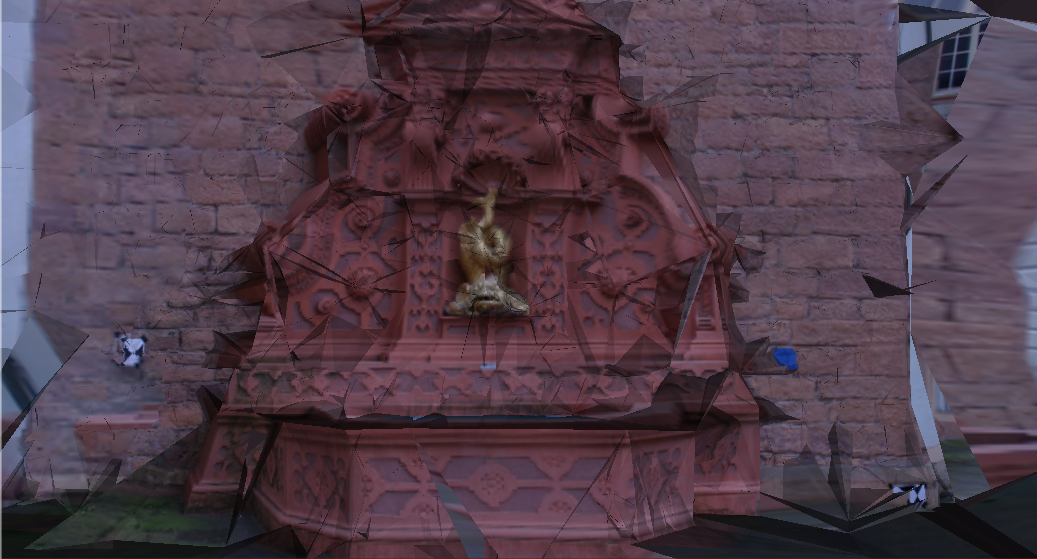
\includegraphics[width=0.25\columnwidth]{./img/first_tex}&
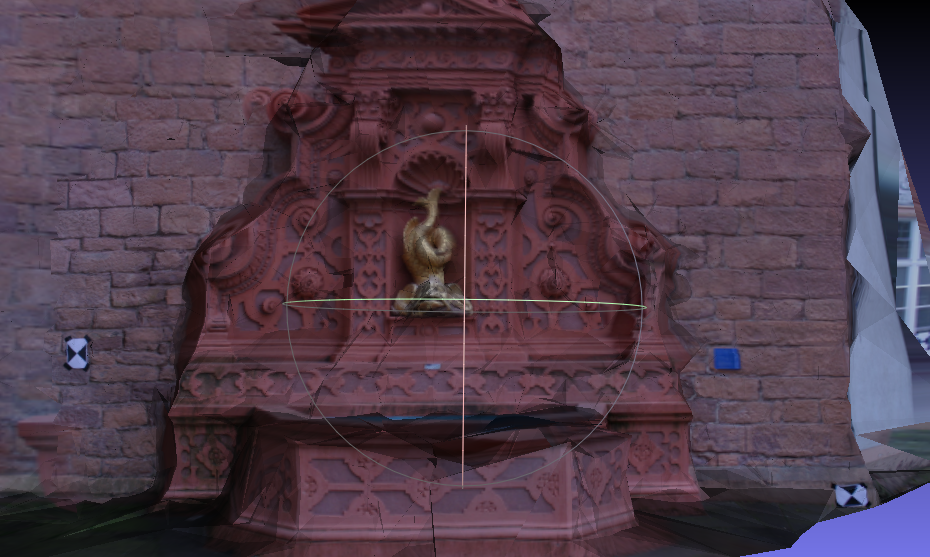
\includegraphics[width=0.25\columnwidth]{./img/myresTex}&
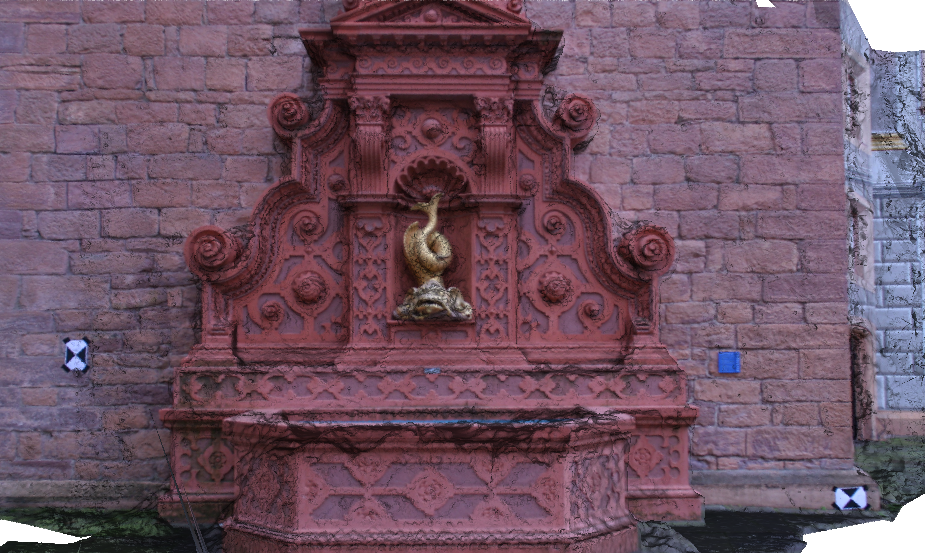
\includegraphics[width=0.25\columnwidth]{./img/photo_mesh_rgb_crop}\\
CMVS &
Initial&
After Mesh&
Photometric\\
Poisson &
manifold&
 Sweeping&
Refinement\\
\end{tabular}
\caption{Images of reconstruction results. First row: depth errors darker blue encodes lower errors, lighter blue encodes higher ones. Second row: untextured reconstruction, third row textured reconstruction.}
\label{fig:fountainIm}
\end{figure}



\begin{figure}[t]
\setlength{\tabcolsep}{1px}
\centering
\begin{tabular}{c}
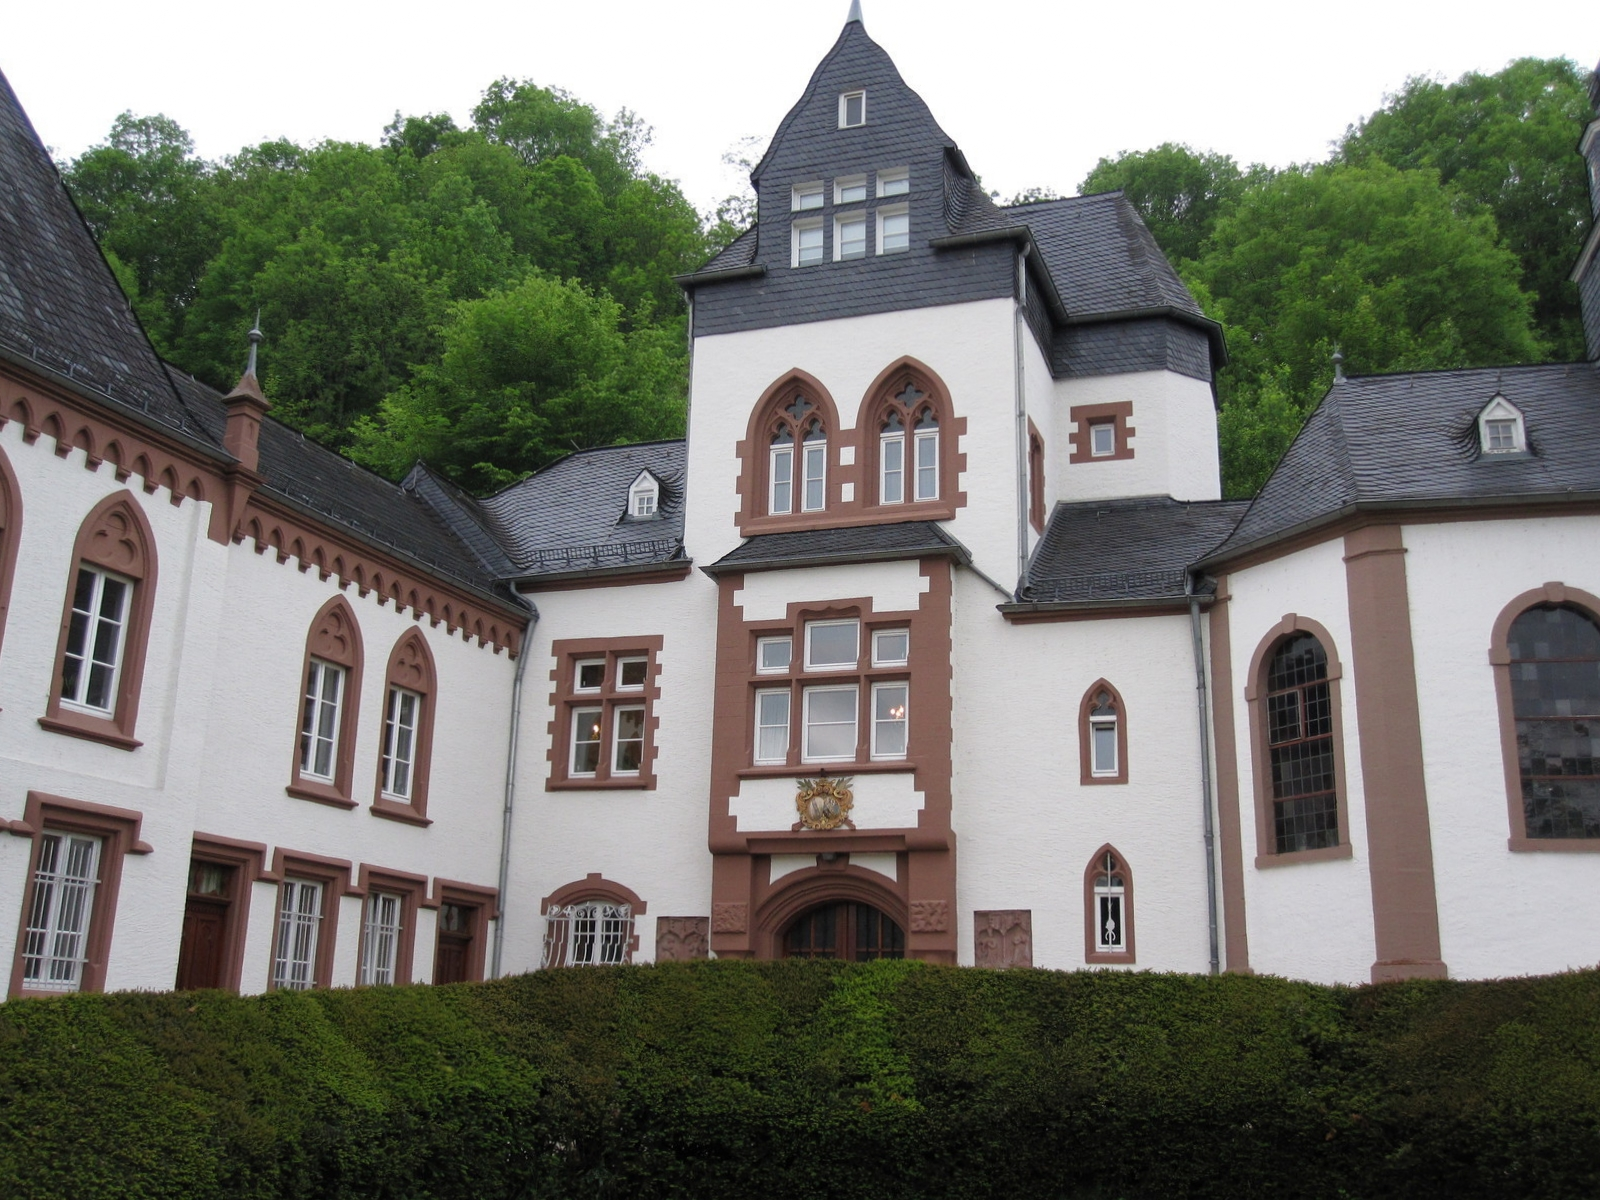
\includegraphics[width=0.8\columnwidth]{./img/dag004}\\
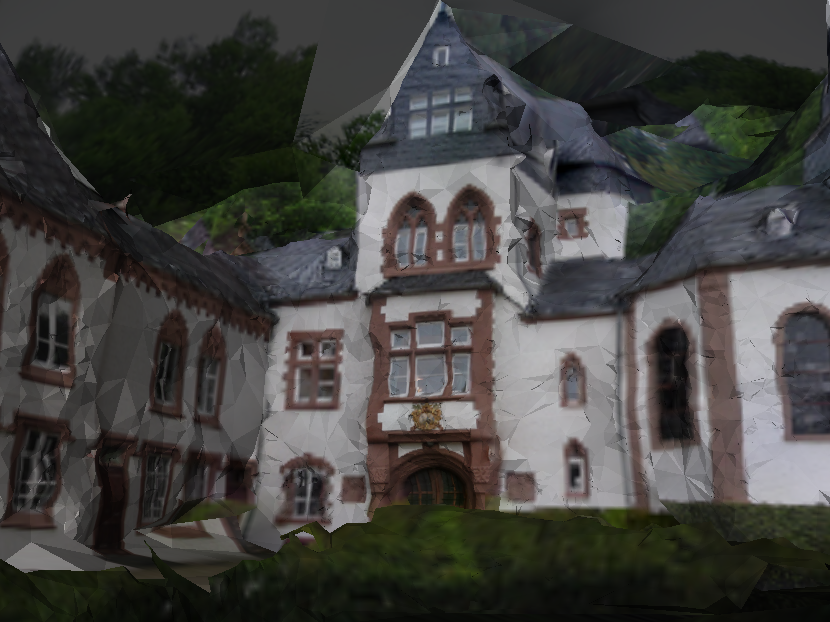
\includegraphics[width=0.8\columnwidth]{./img/d_crop}\\
\end{tabular}
\caption{One frame of the Dagstuhl and reconstruction with the proposed method.}
\label{fig:Dagstuhl}
\end{figure}

\begin{figure}[t]
\centering
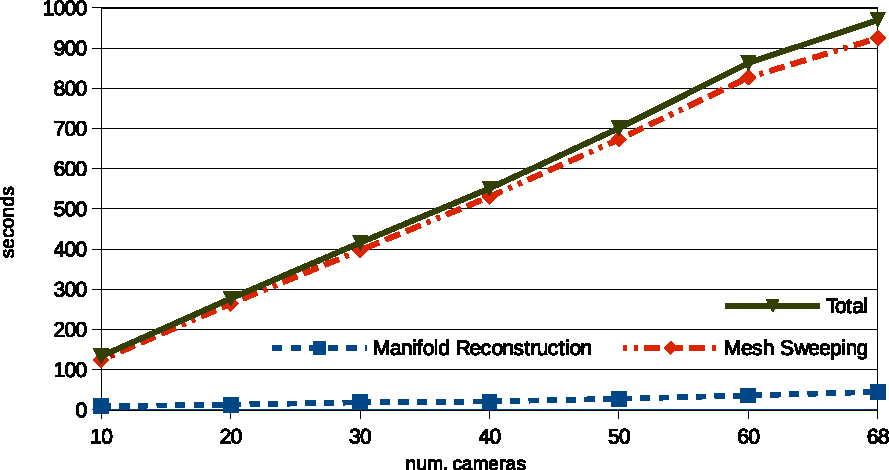
\includegraphics[width=0.99\columnwidth]{./img/timing}
\caption{Processing time with respect to the number of cameras (Dagstuhl dataset).}
\label{fig:scalability}
\end{figure}

